\documentclass[a6paper, 10pt, twoside]{article}
%\usepackage[T1]{fontenc}
\usepackage[british]{babel}
\usepackage[utf8]{inputenc}
\usepackage{float, graphicx,amsmath,amsfonts,cite,enumerate,tabularx}
\usepackage[final]{pdfpages}
\usepackage{wrapfig}
\usepackage[margin=0.3in]{geometry}
\usepackage{sidspaltHack}
\usepackage{digital}

\setlength{\oddsidemargin}{-0.37in}
\setlength{\evensidemargin}{-0.47in}
\setlength{\textwidth}{215pt}

\pagestyle{empty}

\begin{document}
\nysida{13}{1}
\noindent
\chaptertitlenobr{N$\nu$}{Skojiga visor}
\small % TODO: Clean up other smalls in this document.

\begin{center}
\songtitle{$\nu1$}{Lingonben} 
\end{center}
\begin{lyrics}
Bluff och Spark och Tork och Kvark \\
voro sex små dvärgar. \\
En var ful och en var glad\\ 
och en var dum i huvet.
\vspace{5pt}\\ 
Hej, sa Kvark till lille Tork.\\ 
Känner du igelkotten Pilt?\\
Hen som har varit i Paris? \\
Ja, det gjorde Ivar!
\vspace{5pt}\\
Hör du hens lilla runda tass\\ 
när som hen trippar på sitt pass.\\ 
Tripp och trapp och trypa,\\
se hens lilla faster.
\vspace{5pt}\\ 
Tomtefar i skogens brus\\ 
sitter som ett päron.\\
Han har inget eget hus\\ 
allt i sin stora näsa.
\vspace{5pt}\\ 
Söt och blöt är skogens fé.\\ 
Trollen är bjudna hit på te.\\ 
Det lilla trollet pass för det!\\ 
Nu ska mormor bada!
\vspace{5pt}\\ 
Väva och spinna natten lång.\\ 
Prinsen är här i fjorton språng.\\ 
Hipp och hopp och häppla!\\ 
Hästen heter Sverker.

\newpage
\noindent
Stora slottet Drummeldimp\\ 
ligger bortom fjärran.\\
Dit får ingen komma in\\ 
som ej kan baka struvor.
\vspace{5pt}\\ 
Gyllenkrull och Sockertipp!\\ 
Kom, ska vi dansa häxan våt!\\ 
Vill du mig här, så har du nåt!\\ 
Sov du lilla tryne!
\vspace{5pt}\\ 
Kungen är full av stock och sten.\\ 
Skogen är full av lingonben.\\ 
Per är full av tomtar.\\ 
Hur ska lillan orka?\\
\end{lyrics}
\auth{Povel Ramel}

\vspace{35pt}
\begin{figure}[!h]
\centering
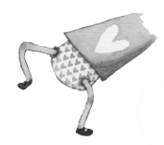
\includegraphics[width=0.5\textwidth]{lingonben.png}
\end{figure}

\nysida{13}{2}
\begin{center}
\songtitle{$\nu2$}{Älska dig själv} 
\mel{Mermaid}
\end{center}
\begin{lyrics}
\small Är du trött på att va' som andra,\\ 
driva med i livets älv?\\ 
Ta och övervinn din mesighet\\ 
och satsa på dig själv!
\vspace{5pt}\\ 
Omvärdera dina värden,\\ 
kasta bort din slavmoral\\ 
och bli krönet på den utveckling\\ 
som har pågått sen neanderthal:
 \vspace{5pt}\\ 
Bli en övermänska, långt bortom gott och ont!\\ 
Övermänni-männi-människan är\\ 
glad och ond som en god James Bond och\\ 
håller blott sej själver kär!
\vspace{5pt}\\  
Du som jämt står sist i krogkön\\ 
och som aldrig får en dans:\\ 
Sluta sjåpa dej, ta piskan fram\\ 
och ge dej själv en chans!
\vspace{5pt}\\  
Hur än allting kommer åter\\ 
gäller blonda bestars bud:\\ 
Du skall upphöjt sträva efter makt\\ 
och du ska va' din egen gud.
\vspace{5pt}\\  
Bli en övermänska, långt bortom gott och ont!\\ 
Övermänni-männi-människan är\\ 
helt komplett, luktar aldrig svett, och\\ 
fri från impotensbesvär.
\end{lyrics}
\auth{Fysikalen Wagner 1986}

\nysida{13}{3}
\begin{center}
\songtitle{$\nu3$}{Balladen om den kaxiga myran} 
\end{center}
\begin{lyrics}
\small Jag uppstämma vill min lyra\\ 
fast det blott är en gitarr\\ 
och berätta om en myra\\ 
som gick ut att leta barr.\\ 
Hen gick ut i morgondiset\\ 
sen hen druckit sin choklad\\ 
och försvann i lingonriset\\ 
$\|$: både mätt och nöjd och glad. :$\|$
\vspace{5pt}\\ 
Det var långan väg att vandra,\\ 
det var långt till närmsta tall.\\ 
Hen kom bort ifrån de andra,\\ 
men var glad i alla fall.\\ 
Femtio meter ifrån stacken,\\ 
just när solnedgången kom,\\ 
hittade hen ett barr på backen\\ 
$\|$: som hen tyckte mycket om. :$\|$
\vspace{5pt}\\  
För att lyfta fick hen stånka,\\ 
hen fick spänna varje lem.\\
Men så började hen kånka\\ 
på det fina barret hem.\\ 
När hen gått i fyra timmar\\ 
kom hen till en ölbutelj.\\ 
Hen såg allting som i dimma,\\ 
$\|$: bröstet hävdes som en bälg. :$\|$
\vspace{5pt}\\  

\newpage
\noindent
Den låg kvar sen förra lördan.\\ 
-Jag ska släcka törsten min,\\ 
tänkte hen och lade bördan\\ 
utanför och klättrade in.\\ 
Hen drack upp den sista droppen,\\ 
som fanns kvar i den butelj.\\ 
Sedan slog hen sig för kroppen\\
$\|$: och skrek ut: -Jag är en älg! :$\|$
\vspace{5pt}\\  
-Ej ett barr jag drar till tjället,\\ 
nej nu ska jag tamigfan\\ 
lämna skogen och istället\\ 
vända uppochner på stan!\\ 
Men hen kom aldrig till staden,\\ 
något spärrade hens stig.\\ 
En koloss där låg bland bladen\\ 
$\|$: och vår myra hejdar sig. :$\|$
\vspace{5pt}\\  
Den var hiskelig att skåda.\\ 
Den var stor och den var grå,\\ 
men vår myra skrek: Anåda,\\ 
om du hindrar mig att gå!\\ 
Hen for ilsket på kolossen,\\ 
som låg utsträckt i hens väg,\\ 
men vår myra kom ej loss sen.\\ 
$\|$: Hen satt fast som i en deg. :$\|$
\vspace{5pt}\\  
Sorgligt slutar denna sången.\\ 
Myran stretade och drog,\\ 
men kolossen höllen fången\\ 
tills hen svalt ihjäl och dog.\\ 
Undvik alkoholens yra.\\ 
Du blir stursk, men kroppen loj\\ 
och om du är född till myra:\\ 
$\|$:Brottas aldrig med ett TOY! :$\|$ 
\end{lyrics}

\nysida{13}{4}
\begin{center}
\songtitle{$\nu4$}{Nikolajev} 
\mel{Rysslands nationalsång}
\end{center}
\begin{lyrics}
\small Mitt namn är Nikolajev,\\ 
kosmonaut från Sovjet.\\ 
Jag flyger runt jorden\\ 
i min rymdraket.\\ 
Och där ska jag stanna i 84 varv\\ 
för det har Chrustjev sagt,\\ 
men det tycker jag är larv.
\vspace{5pt}\\ 
Jag längtar hem, hem till min planet.\\ 
Till fru och barn därhemma i Sovjet.\\ 
Men mest utav allt längtar jag till ett rum\\ 
med ett hjärta på dörren.\\ 
Jag längtar hem till min planet.\\ 
Till fru och barn därhemma i Sovjet.
\vspace{5pt}\\ 
Min kapsel innehåller\\ 
många instrument.\\ 
Ja, mycket av sådant\\ 
som ännu ej är känt.\\ 
Men lika förbannat, vad du än tror:\\ 
jag glömde gå på muggen\\ 
innan jag for.
\vspace{5pt}\\ 
Jag längtar hem...\\
\end{lyrics}

\begin{figure}[!h]
\hfill

\includegraphics[width=0.35\textwidth]{rymdraket.png}
\end{figure}

\nysida{13}{5}
\begin{center}
\songtitle{$\nu5$}{Danse Macabre} 
\mel{Vårvindar friska}
\end{center}
\begin{lyrics}
\small Runt kring vår stuga\\ 
smådjävlar sluga\\ 
tassa så tyst med bockfot och svans.\\ 
Varulvar yla,\\ 
isande kyla\\ 
sveper i dimma fanstygets dans.
\vspace{5pt}\\ 
Bäva, o fränder, lyssna och hör\\ 
vrålen från gast som osalig dör.\\ 
Satan hen skrattar,\\ 
flaskan hen fattar,\\ 
super tills dagen gryr.
\vspace{5pt}\\ 
Gastar och spöken\\ 
skymtar i kröken.\\ 
Dödingar släpar ruttnande lik.\\ 
Benrangel skramla,\\ 
spökhänder famla,\\ 
kväva din strupes rosslande skrik.
\vspace{5pt}\\ 
Helvetets alla fasor släppts loss,\\ 
Fan rider här med hela sin tross.\\ 
Göm dig i stugan,\\ 
du har fått flugan,\\ 
dille det blir din lott.\\
\end{lyrics}
\auth{Carl-Erik Carlstedt, CTH}

\nysida{13}{6}
\begin{center}
\songtitle{$\nu6$}{Katten} 
\mel{Glad såsom fågeln}
\end{center}
\begin{lyrics}
\small Glad åt en fågel i morgonstunden\\ 
går hen på jakt i den friska natur.\\ 
Lärkan hen ratar, men trasten i lunden\\ 
lyckas hen fånga, nej tänk en sån tur!
\vspace{5pt}\\ 
Se hur de fjädrade vingarne små\\ 
hoppa och slå, hoppa och slå.\\ 
Vänliga tarmar kring buskar och grenor\\ 
se, hur det spritter i muskler och senor\\ 
av liv och av dans? Nej, trasten är hens,\\
och hen kröker sin listiga svans\\ 
jakten går som en dans\\
uti vår-sol-ens glans! \\
\end{lyrics}
\begin{center}
\songtitle{$\nu7$}{Undulaten} 
\mel{Med en enkel tulipan}
\end{center}
\begin{lyrics}
\small Jag är en liten undulat,\\
som får så dåligt med mat,\\
för dom jag bor hos,\\
för dom jag bor hos,\\
dom är så snåla.\\
Dom ger mig fisk varenda dag,\\
men det vill jag inte ha,\\
jag vill ha rödvin,\\
jag vill ha rödvin,\\
och Gorgonzola.
\end{lyrics}

\nysida{13}{8}
\begin{center}
\songtitle{$\nu8$}{Bakfyllosofen} 
\mel{34:an}
\end{center}
\begin{lyrics}
\small Eskimåer jagar valross.\\
Alla tyskar jagar älg.\\
Pedofiler jagar småglin.\\
Vilken värld, ja skål och svälj.
\vspace{5pt}\\
Uti skogen finns det blåbär.\\
På balkongen står en stol.\\
Uti stolen sitter jag.\\
Jag har vatt bakfull sen i fjol.\\
\vspace{5pt}\\
Om du hör nånting som tickar,\\
kan det kanske va en bomb.\\
Om det är en väckarklocka,\\
bara vänd och somna om.\\
Om du har en liten tax\\
och så en fet gul undulat.\\
$\|$:Ja då hopar sig problemen,\\
en kan inte ge dem samma mat. :$\|$
\end{lyrics}
\auth{Fysiksektionen, LTH}
\begin{center}
\songtitle{$\nu9$}{Mellansup} 
\mel{Fredagsmys }
\end{center}
\begin{lyrics}
\small Det är dags för mellansup,\\
om det så är det sista jag gör.\\
Det är dags för mellansup,\\ 
hoppas inte att toastmastern stör.\\
Nu är det slut på versen,\\
det är dags för mellansup!
\end{lyrics}
\auth{Fysiksektionen, LTH}

\nysida{13}{10}
\begin{center}
\songtitle{$\nu10$}{Kanta Studjosi} 
\mel{Studentsången}
\end{center}
\begin{lyrics}
\small Kantom studjosi extarbon sjur!\\
Lassom galejan in spring juvenar,\\
nock funkar kardan kum san' bravur,\\
kaj futura blondina üst var.\\
Nolla furii\\
in va psykosan sit,\\
esperan v'ami,\\
promissan va kredit,\\
kum voj knopa bandage in plantage,\\
kvo dulkissan diploma florit,\\
kvo dulkissan diploma florit,\\
Hojlah!
\end{lyrics}
\vspace{-16pt}\\
\auth{magister Ludvig Hagwald, Grönköping}
\begin{center}
\songtitle{$\nu11$}{Indialand} 
\end{center}
\begin{lyrics}
\small I Indialand, bak Himalayas rand,\\
där händer det konstiga saker ibland.\\
Se'n urminnes tider fanns heliga kon.\\
Nu har den bytts ut mot en Boforskanon.
\vspace{5pt}\\
Det började så, en man vid namn Gandhi\\
sa: "Vi ska ha något med mycket krut i.\\
Det som finns i Sverige behöver vi nu,\\
säg, hette den inte Haubits 77?"
\vspace{5pt}\\
Han trollade så att ett konto i Schweiz\\
försvann och bluvanerna sade hej-svejs,\\
för tydligen har inte papper fyllts i\\
och Roine förstår lika lite som vi\\
Woine woine Roine woine Roine...
\end{lyrics}
\auth{Karl Lindén}

\nysida{13}{12}
\begin{center}
\songtitle{$\nu12$}{Zwampen} 
\end{center}
\begin{lyrics}
\small Jag gillar inte höghus,\\
sten och lätt betong.\\
Jag trivs inte i stan\\
för den är grå och trång.
\vspace{5pt}\\
Jag vill bo i en svamp, annars får jag kramp. (svamp)\\
Det finns hopp för min kropp, i en mullig sopp. (svamp)\\
Kom ikväll och var snäll, till min kantarell. (svamp)\\
Titta in och ta ton, i min champinjon. (svamp)
\vspace{5pt}\\
Jag vill bo i skogen,\\
i lugn och rymd och ljus.\\
Och sitta framför svampen\\
och höra tallens sus.
\vspace{5pt}\\
Jag vill bo i en svamp, annars får jag kramp. (svamp)\\
Det finns hopp för min kropp, i en mullig sopp. (svamp)\\
Kom ikväll och var snäll, till min kantarell. (svamp)\\
Titta in och ta ton, i min champinjon. (svamp)
\vspace{5pt}\\
Tiderna är hårda,\\
livet är en kamp.\\
Det känns mycket bättre\\
om jag har min svamp.
\vspace{5pt}\\
Jag vill bo i en svamp, annars får jag kramp. (svamp)\\
Det finns hopp för min kropp, i en mullig sopp. (svamp)\\
Kom ikväll och var snäll, till min kantarell. (svamp)\\
Titta in och ta ton, i min champinjon. (svamp)
\vspace{5pt}\\
\end{lyrics}
\auth{Electric Banana Band}

\nysida{13}{13}
\begin{center}
\songtitle{$\nu13$}{Lumberjack song} 
\small\textit{\textbf{Leader} / Mounties}
\end{center}
\begin{lyrics}
\small 
\textbf{I'm a lumberjack\\ 
And I'm O.K\\ 
I sleep all night\\ 
And I work all day}
\vspace{5pt}\\ 
He's a lumberjack\\ 
And he's O.K\\ 
He sleeps all night\\ 
And he works all day
\vspace{5pt}\\
\textbf{I cut down trees\\ 
I eat my lunch\\ 
I go to the lavatory\\ 
On Wednesday I go shopping\\ 
And have buttered scones for tea}
\vspace{5pt}\\ 
He cuts down trees\\ 
He eats his lunch\\ 
He goes to the lavatory\\ 
On Wednesday he goes shopping\\ 
And has buttered scones for tea 
\vspace{5pt}\\
He's a lumberjack\\ 
And he's O.K\\ 
He sleeps all night\\
And he works all day
\newpage
\noindent
\textbf{I cut down trees\\ 
I skip and jump\\ 
I like to press wild flowers\\ 
I put on women's clothing\\ 
And hang around in bars}
\vspace{5pt}\\ 
He cuts down trees\\ 
He skips and jumps\\ 
He likes to press wild flowers\\ 
He puts on women's clothing\\ 
And hangs around in bars
\vspace{5pt}\\ 
He's a lumberjack\\ 
And he's O.K\\ 
He sleeps all night\\ 
And he works all day
\vspace{5pt}\\ 
\textbf{I cut down trees\\ 
I wear high heels\\ 
Suspenders and a bra\\ 
I wish I'd been a girlie\\ 
Just like my dear Papa}
\vspace{5pt}\\ 
He cuts down trees\\ 
He wears high heels\\ 
(spoken rather than sung)\\ 
Suspenders ..... and a bra?\\ 
That's shocking!\\ 
That's rude...tuttut...tut...tut
\end{lyrics}
\auth{Monty Python's Flying Circus}

\nysida{13}{14}
\begin{center}
\songtitle{$\nu14$}{Under en filt i Madrid} 
\end{center}
\begin{lyrics}
\small Under en filt i Madrid\\ 
där ligger en flicka på glid.\\ 
Tittar på mannen bredvid\\ 
under en filt i Madrid.
\vspace{5pt}\\ 
Bakom ett berg i Geneve\\ 
där får en moder ett brev\\
från hennes dotter på glid\\ 
under en filt i Madrid.
\vspace{5pt}\\  
Framför en stolpe i Bonn\\ 
sitter det nu inte nån.\\ 
Bara en tom La Garonne\\ 
framför en stolpe i Bonn.
\vspace{5pt}\\  
Men, där i vindarnas drev\\ 
fladdrar ett brev från Geneve,\\ 
postat en gång i Bretagne,\\ 
doftande billig Champagne.
\vspace{5pt}\\  
På en bordell i Borås\\ 
smörjer en herre sitt krås.\\ 
Bakom ett skjul i Tasjkent\\ 
där står ett fönster på glänt.
\vspace{5pt}\\  
Någon har kastat ett skal\\ 
genom en jak i Nepal.\\ 
Ingenting är som det skall\\ 
solen är blott en marschall. 
\newpage
\noindent
Och själv är jag blott en kostym.\\ 
Mamma är bara parfym.\\ 
Pappa förspiller sin tid\\ 
under en filt i Madrid.
\vspace{5pt}\\  
Under ett lakan i Prag\\ 
ligger en kvinna och jag.\\ 
Sängen är full av resår\\ 
sången jag sjunger är svår.
\vspace{5pt}\\  
Omöjlig att ta sig ur,\\ 
jag vete fan inte hur.\\ 
Orden får snart inte rum,\\ 
jag får väl sjunga mig stum!
\vspace{5pt}\\  
Tonerna trängs i min gom,\\ 
sätt mig på tåget till Rom!\\ 
Låt mig få sluta min tid\\ 
under en filt i Madrid! 
\end{lyrics}
\auth{Claes Eriksson}
\vspace{25pt}
\begin{figure}[!h]
\center
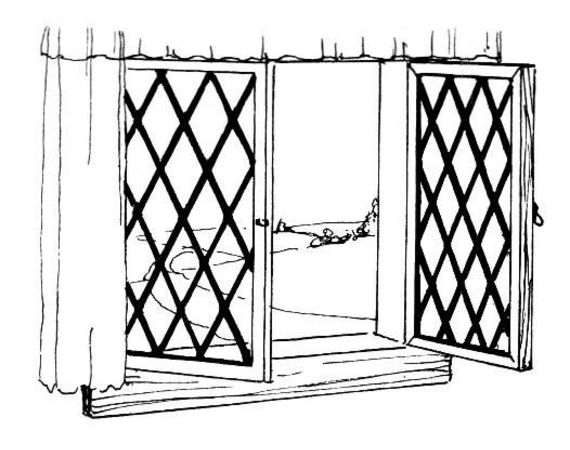
\includegraphics[width=0.5\textwidth]{fonster.png}
\end{figure}

\nysida{13}{15}
\noindent
\begin{center}
\songtitle{$\nu15$}{Hallen luta}
\mel{Hallelujah}
\end{center}
\begin{lyrics} 
\small Jag minns knappt hur jag tog mig hem, \\
klockan var minst kvart i fem \\
när jag stod utanför min egen våning. \\
Jag lyfte upp min nyckelring \\
och haja nästan ingenting, \\
när dörren öppnas står min hall och lutar. \\
Hallen luta, hallen luta, \\
hallen luta, hallen lu-u-u-u-uta. \\
\vspace{5pt}\\
Jag minns knappt julen nittitre \\
min bror var där och syster me, \\
å snyggingen i rött satt alldles bredve. \\
Vi drack vår glögg och pratade \\
min dejt blev trött och schappade \\
Så jag fick mera tid för han den röde. \\
Han i luva, han i luva, \\
han i luva, han i lu-u-u-u-uva. \\
\vspace{5pt}\\
Fredagen har mer att ge \\
än räkor snask och en TV. \\
En kan ju hyra film och DVD. \\
Å vill en ha något riktigt bra \\
så kan en faktiskt bara ta \\
en film som vunnit Oscar åt en Berry. \\
Halle Berry, Halle Berry, \\
Halle Berry, Halle Be-e-e-e-erry. \\
\end{lyrics}

\nysida{13}{16}
\begin{center}
\songtitle{$\nu16$}{Styrman Karlssons äventyr med porslinspjäsen} 
\end{center}
\vspace{-5pt}
\begin{lyrics}
\small Stackars styrman Karlsson hade otur,\\
skulle gå på flottans fest igår.\\
När hen skulle snöra på sej skorna\\
måttade hen fel med sina tår.
\vspace{5pt}\\
Hen satte foten i sin potta\\
och kunde inte komma loss!\\
Hens fot är storlek förtiåtta\\
och den var alltför stor förstås.
\vspace{5pt}\\
Hen putsa upp den med skokräm,\\
så att den glänste svart och fin.\\
Och snart på balen sågs hen dansa\\
med sin sko utav porslin.
\vspace{5pt}\\
Hen hade foten i en potta\\
men så hen svängde sina ben!\\
Så bra att chefen för vår flotta\\
utnämnde Karlsson till kapten.
\vspace{5pt}\\
Nu är kapten Karlsson havets fasa,\\
alla sjöpiraters stora skräck.\\
Över vattnet hör en tydligt ekot\\
av hens steg, när hen går kring på däck.
\vspace{5pt}\\
Ja hen går med foten i en potta\\
för hen har aldrig kommit loss.\\
Och så'na sparkar hen kan måtta,\\
när hen i drabbningarna slåss!
\vspace{5pt}\\
En gång så föll hen från skutan\\
och tänkte: "Nu så blir jag våt.\\
Hur ska jag komma hem till Sverige?\\
Jag har ju inte någon båt."

\nysida{13}{17}
\noindent
Hen hade foten i en potta.\\
I denna seglade hen hem.\\
Och möttes av sin fru Charlotta,\\
som också har sin fot i kläm.\\
(i en byrålåda i en chiffonjé, olé!)
\end{lyrics}
\begin{center}
\songtitle{$\nu17$}{Sjung om Fru Svenssons lyckliga karl} 
\end{center}
\begin{lyrics}
\small Sjung om fru Svenssons lyckliga karl,\\
låt honom plöja i ungdomens fåror.\\
Fem gamla hjärtan i sprit har jag,\\
å' en ljus elefant i ett snår.\\
Inga stoppar den,\\
i vårat linneskåp.\\
Loppor tär vår vän, \\
som idisslar en sko \\
när vi snyta en rund liten hund.\\
$\|$: Där den här lilla bagaren bor. :$\|$\\
Hursa?
\end{lyrics}

\begin{center}
\songtitle{$\nu18$}{Jesus lever}
\mel{Sånt är livet}
\end{center}
\begin{lyrics}
\vspace{-5pt}
\small Jesus lever, han bor i Skövde\\
Han kör en Volvo och han är gift\\
Han har en villa med rododendron\\
Han sparar pengar och jobbar skift\\
\vspace{5pt}\\
Redan på lekis var han märklig\\
Han ville inte leka krig\\
Men när hans kompis, Knut, blev skjuten\\
så lät han Jesus uppväcka sig\\
\vspace{5pt}\\
Jesus lever, han bor i Skövde...\\
\vspace{5pt}\\
Han gick i skolan, som alla andra\\
Han var rätt duktig på gymnastik\\
å vilken kille han gick på vatten\\
en gång så gick han till Reykjavik\\
\vspace{5pt}\\
Jesus lever, han bor i Skövde...\\
\vspace{5pt}\\
I sina tonår så var han poppis\\
Och han blev bjuden på varje fest\\
Å vilken kille, han fick ju vatten\\
att bli till rusdryck utan jäst\\
\vspace{5pt}\\
$\|$: Jesus lever, han bor i Skövde... :$\|$\\
\end{lyrics}
\begin{center}
\songtitle{$\nu37,5$}{Temperaturen} 
\end{center}
\begin{lyrics}
\small Temperaturen är hög uti kroppen,\\ 
närmare 40 än 37,5.\\ 
Men så skall det vara när ångan är oppe,\\ 
och så är fallet uti detta nu!\\ 
$\|$: Det rullar, det rullar, vi rullar, vi rullar,\\ 
vi rullar, vi rullar, vi rullar, å hej! :$\|$\\
Å framåt och bakåt...\\
Å höger och vänster...\\ 
August... och Lotta... 
\end{lyrics}
\end{document}